\section{Memory Models}

\subsection{Introduction}

The target we consider at present,
is either the LEON GR172RC or LEON GR740 (SPARC) processor,
running with the Total Store Order (TSO) memory model.

\subsection{SPARC Architecture Manual, Version 8}

\subsubsection{SPARC v8 Memory Model}

Chapter 6, p59.


p61:

Memory is byte-addressed, with halfword accesses aligned on 2-byte boundaries,
word accesses aligned on 4-byte boundaries,
and doubleword accesses aligned on 8-byte boundaries.
The largest datum that is atomically read or written
by memory hardware is a doubleword.
Also, memory references to different bytes, halfwords,
and words in a given doubleword are treated for ordering purposes as
references to the same location.
Thus the unit of ordering for memory is a doubleword.

p62:

The distinction
between instruction fetches and instruction loads is important;
confusing the two will lead to incorrect conclusions about the memory model.

The FLUSH instruction synchronizes instruction fetches
with data loads and stores:
when a processor executes FLUSH A,
the data corresponding to location A is removed
from the IBufs of all processors in the system
some time after the execution of the FLUSH.
An implementation may choose to flush any portion of IBuf
as long as location A is included.

\subsubsection{Total Store Ordering  (TSO)}

p64

Total Store Ordering guarantees that the store, FLUSH,
and atomic load-store instructions of all processors
appear to be executed by memory serially
in a single order called the memory order.
Furthermore, the sequence of store, FLUSH,
and atomic load-store instructions in the memory order
for a given processor
is identical to the sequence in which they were issued by the processor.

Stores, FLUSHes, and atomic load-stores issued by a processor
are placed in its dedicated Store Buffer,
which is FIFO.

A load by a processor first checks its Store Buffer
to see if it contains a store to the same location
(atomic load-stores do not need to be checked for
because they block the processor).
If it does,
then the load returns the value of the most recent such store;
otherwise the load goes directly to memory.
Since not all loads go to memory,
loads in general do not appear in the memory order.
A processor is blocked from issuing further memory operations until the load returns a value.

An atomic load-store (SWAP or LDSTUB) behaves like both a load and a store.
It is placed in the Store Buffer like a store,
and it blocks the processor like a load.
In other words,
the atomic load-store blocks until the store buffer is empty
and then proceeds to memory.
A load therefore does not need to check
for atomic load-stores in the Store Buffer
because this situation cannot arise.

pp64-65:

When memory services an atomic load-store,
it does so atomically:
no other operation may intervene between
the load and store parts of the load-store.

\newpage
\subsubsection{Formal Specification of the Memory Model}

Appendix K, p281.

Some notation:

\begin{tabular}{|c|l|}
  \hline
  L & data load
\\\hline
  S & data store
\\\hline
  [L \iseq\ S] & atomic load-store
\\\hline
  F & FLUSH
\\\hline
  IF & instruction fetch
\\\hline
  IL & instruction load
\\\hline
  $X_a^i$ & processor $P^i$ does $X$ on address $a$.
\\\hline
  S\#n & stores value $n$
\\\hline
 \textbf{Val}[$L_a^i$] & value returned by $L_a^i$.
\\\hline
 \textbf{Val}[$S_a^i$] & value in locn. $a$ immediately after $S_a^i$.
\\\hline
  $SOp$ & $S$ or $F$
\\\hline
  $Op$ & $L$, $S$ or $F$, and \textbf{not} $[L \iseq S]$
\\\hline
\end{tabular}

Addresses refer to doublewords, which is the granularity of all of this.

\begin{description}
  \item [memory order]
    A partial order ($\leq$) describing the order
    in which memory performs the operations.
  \item[program order]
    A total order ($\iseq^i$), one for each processor $i$,
    giving its sequence of instruction execution.
\end{description}

p283:

TSO guarantees that the store, FLUSH,
and atomic load-store instructions of all processors
appear to be executed by memory serially
in a single order called the memory order $\leq$ .
It further guarantees that
the sequence of these instructions for each processor $i$
is the same in the orders $\iseq^i$ and $\leq$ .

Axioms:

\paragraph{Order}

All $S$ and $F$ appear in the memory order
(i.e., they form a total sub-order of the partial memory order).

\begin{equation*}
  (SOp_a^i \leq SOp_b^j) \lor (SOp_b^j \leq SOp_a^i)
\end{equation*}

\paragraph{Atomicity}

In [L \iseq S], $L$ issues before $S$, so $L \leq S$,
and no other $S'$ occurs between $L$ and $S$.

\begin{equation*}
  [L_a^i \iseq S_a^i]
  \implies
  (L_a^i \leq S_a^i)
  \land
  (\forall SOp_b^j
   \bullet
     SOp_b^j \leq L_a^i \lor S_a^i \leq SOp_b^j
   )
\end{equation*}


\paragraph{Termination}

All stores and loads terminate.
A store to any location
will always be read after a finite number of loads from that location.

\begin{equation*}
   S_a^i \land (L_a^j)^\infty
   \implies
   \exists L_a^j \in (L_a^j)^\infty
   \bullet
   S_a^i \leq L_a^j
\end{equation*}

\paragraph{Value}

Load value is always that of the most recent store.

\begin{equation*}
   \textbf{Val}[L_a^i]
   =
   \textbf{Val}
      [ S_a^j
        |
        S_a^j
        =
        Max_{\leq}
          [ \setof{S_a^k | S_a^k \leq L_a^i}
            \cup
            \setof{S_a^i | S_a^i \iseq L_a^i}
          ]
      ]
\end{equation*}

\paragraph{LoadOp}

Any operation issued on a given processor after an $L$
is later in order $\leq$.

\begin{equation*}
   L_a^i \iseq Op_b^i
   \implies
   L_a^i \leq Op_b^i
\end{equation*}

\paragraph{StoreStore}

Operations $S$ and $F$ from a given processor
appear in the same order in memory.

\begin{equation*}
   SOp_a^i \iseq SOp_b^i
   \implies
   SOp_a^i \leq SOp_b^i
\end{equation*}


\subsection{Gaisler GR740 Memory Model Details}

From presentation (\url{https://www.gaisler.com/doc/gr740/GR740-OVERVIEW.pdf}),
 L1 cache per processor
- multi-set, write-through, LRU/LRR/RND policies.

L2 cache from shared processor bus to outside world.
Highly configurable (can even act as RAM!)

From latest specification document
(\url{https://www.gaisler.com/doc/gr740/GR740-UM-DS-2-4.pdf}):

Eight register windows

Write through data cache with bus-snooping for coherency.

p58:

The data cache contains a write buffer
able to hold a single 8,16,32, or 64-bit write.

p63:

When using caches with snooping (and with physical tags if using the MMU),
the shared memory will act
according to the slightly weaker SPARC Total Store Order (TSO) model.
The TSO model is close to SC,
except that loads may be reordered before stores coming from the same CPU.
The stores and atomics are conceptually placed in a FIFO
(see the diagrams in the SPARC standard)
and the loads are allowed to bypass the FIFO
if they are not to the same address as the stores.
Loaded data from other addresses may therefore be either older or newer,
with respect to the global memory order,
than the stores that have been performed by the same CPU.


\subsection{Isabelle/HOL Formalisation}

This is a paper by Zh\'{e} H\'{o}u, David San\'{a}n and others,
found at \url{https://link.springer.com/article/10.1007/s10817-020-09579-4}.


More notation!

p585:

\subsubsection{Operation Blocks}

"memory operation blocks"
are groups of instructions,
and each group contains at most one memory operation.

"program block" is a list of instructions where the last instruction
is a memory instruction (load, store, etc.).

p586:

A program is a list of program blocks,
with the last being allowed to not have any memory operation.

An atomic load-store is modelled by two consecutive program blocks.

Each programming block can be uniquely identified
\begin{equation*}
  M_{block} = "id \implies block"
\end{equation*}
A block is a triple $\langle i,p,id \rangle$,
where $i$ is the list of instructions, $p$ is the processor number,
and $id$ is optional,
and is mainly used to allow an atomic store block
to refer to the corresponding atomic load block.

\subsubsection{Program Order}

"program order" is the order in which a processor executes instructions.
A program order $PO$ maps a processor number $p$ to its list of instructions.
\begin{equation*}
   PO = "p \implies id\;list"
\end{equation*}

\paragraph{Program Order Before}

$id_1;^p_{PO} id_2$ iff $id_1$ is before $id_2$ in $(PO~p)$.

When $PO$ and $p$ are obvious, write $id_1;id_2$.

Note that $id_1;id_2$ means both ids are on the same processor.



\subsubsection{Memory Order Before}

p588:

Let $x$ denote a sequence of ids from the execution of processor $i$%
\footnote{Note the (confusing) notation change here.
In the previous section, $p$ was used as a processor number. }
as seen by memory.

p589:

\paragraph{Memory Order Before}
\begin{eqnarray*}
   id_1 <_x id_2
   &\equiv&
     \IF (id_1 \in x) \land (id_2 \in x) \THEN
\\&& \quad \IF id_1 \textrm{ is before } id_2 \textrm{ in } x
              \THEN true \ELSE false
\\&& \ELSE
\\&& \quad \IF id_1 \in x \THEN true
\\&& \quad \ELSE \IF id_2 \in x \THEN false
\\&& \quad \ELSE undefined
\end{eqnarray*}

\subsubsection{TSO Axioms}

\paragraph{Axiom Order}

\begin{eqnarray*}
\lefteqn{\mathbf{Order}~id~id'~x~ M_{block} \equiv {}}
\\&& id \neq id' \land {id,id'} \subseteq x
\\&& id,id' \mbox{are store/atomic-store blocks}
\\&& \implies
\\&& (id <_x id') \lor (id' <_x id)
\end{eqnarray*}

\paragraph{Axiom Atomicity}

\begin{eqnarray*}
\lefteqn{\mathbf{Atomicity}~id_l~id_s~PO~x~ M_{block} \equiv {}}
\\&& id_l \neq id_s \land \{id_l,id_s\} \subseteq (PO~p) \textrm{ for some }p
\\&& id_l~(id_s) \textrm{ is an atomic load (store) block}
\\&& id \in x \land id \neq id_s
\\&& id \mbox{ is a store/atomic-store block}
\\&& id_l ; id_s
\\&& \implies
\\&& id_l <_x id_s
\\&& (id <_x id_l) \lor (id_s <_x id)
\end{eqnarray*}

\paragraph{Axiom Termination}

\begin{eqnarray*}
\lefteqn{\mathbf{Termination}~id~PO~x~ M_{block} \equiv {}}
\\&& \exists p \bullet id \in (PO~p)
                       \land id
                       \mbox{ is store/atomic-store}
\\&& \implies
\\&& id \in x
\end{eqnarray*}

\paragraph{Axiom Value}

\begin{eqnarray*}
\lefteqn{\mathbf{Value}~p~id~addr~PO~x~ M_{block}~state \equiv {}}
\\&& S_1 = \mbox{ store/atomic-stores before }
           id \in PO
           \mbox{ writing to }
           addr
\\&& S_2  = \mbox{ store/atomic-stores before }
           id \in <_x
           \mbox{ writing to }
           addr
\\&& id' = last_{<_x}(S_1 \cup S_2)
\\&& \implies
\\&& Lval_{id} = Sval_{id'}
\end{eqnarray*}
Here $Lval_{id}$ denotes the value loaded by $id$,
and $Sval_{id'}$ denotes the value stored by $id'$.

\paragraph{Axiom LoadOp}

p590:

\begin{eqnarray*}
\lefteqn{\mathbf{Load}~id~id'~PO~x~ M_{block} \equiv {}}
\\&& id \mbox{ is a load/load-atomic block}
\\&& id ; id'
\\&&\implies
\\&& id <_x id'
\end{eqnarray*}

\paragraph{Axiom StoreStore}

\begin{eqnarray*}
\lefteqn{\mathbf{StoreStore}~id~id'~PO~x~ M_{block} \equiv {}}
\\&& id,id' \mbox{are store/atomic-store blocks}
\\&& id;id'
\\&&\implies
\\&& id <_x id'
\end{eqnarray*}

\subsubsection{Operational TSO Model}

p590:

Notation:\\
\begin{tabular}{|c|l|}
  \hline
  $exe_{id}$ & executes all instructions in block $id$
\\\hline
  $exe^{pre}_{id}$ & executes all instructions, except for the last, in block $id$
\\\hline
  $exe^{last}_{id}$ & executes the last instruction in block $id$
\\\hline
  $type_{id}$ & type of block $id$ $(ld,ald,st,ast,non)$.
\\\hline
  $x@x'$ & $x$ concatenated with $x'$
\\\hline
  $\langle x,s\rangle$
  & (past) operation sequence $x$ paired with (current) state $s$
\\\hline
  $x,s \rightsquigarrow x',s'$ & operation mapping $\langle x,s\rangle$ to $\langle x',s'\rangle$
\\\hline
\end{tabular}

\paragraph{Load Rule}

pp590--591:

\begin{description}
  \item [Premises]~
    \begin{itemize}
      \item $type_{id} = ld$
      \item $\forall id' \bullet
              (id';id) \land type_{id'} \in \{ld,ald\}
              \implies
              id' \in x
            $
    \end{itemize}
  \item [Operation]~
    \begin{itemize}
      \item $x' = x@[id]$
      \item From $s$ , execute $id$ until last instruction, obtain $s_1$.
      \item From $s_1$ get load value
      \item From $s_1$ execute last instruction, obtain $s'$
    \end{itemize}
\end{description}

$$
\inferrule
  { type_{id}=ld
    \\
    \forall id' \bullet
            (id';id) \land type_{id'} \in \{ld,ald\}
            \implies
            id' \in x
  }
  {x,s \rightsquigarrow x@[id],(exe_{id}^{last} LVal_{id} (exe_{id}^{pre}s))}
$$

\paragraph{Store Rule}

p591:

\begin{description}
  \item [Premises]~
    \begin{itemize}
      \item $type_{id} = st$
      \item $flag_{atom} = undefined$
      \item $ \forall id' \bullet
              (id';id) \land type_{id'} \in \{ld,ald,st,ast\}
              \implies
              id' \in x
            $
    \end{itemize}
  \item [Operation]~
    \begin{itemize}
      \item $x' = x@[id]$
      \item From $s$ execute $id$, obtain $s_1$
      \item From $s_1$ write value to memory, obtain $s'$
    \end{itemize}
\end{description}

$$
\inferrule
  {type_{id} = st \\ flag_{atom} = undefined
   \\\\
   \forall id' \bullet
           (id';id) \land type_{id'} \in \{ld,ald,st,ast\}
           \implies
           id' \in x}
  {x,s \rightsquigarrow x@[id],(Wmem~id~(exe_{id}~s))}
$$

\newpage
\paragraph{Atomic Load Rule}


\begin{description}
  \item [Premises]~
    \begin{itemize}
      \item $type_{id} = als$
      \item $flag_{atom} = undefined$
      \item $ \forall id' \bullet
              (id';id) \land type_{id'} \in \{ld,ald,st,ast\}
              \implies
              id' \in x
            $
    \end{itemize}
  \item [Operation]~
    \begin{itemize}
      \item $x' = x@[id]$
      \item From $s$ execute $i$ until last instruction, obtain $s_1$
      \item From $s_1$ get value via $Lval_{id}$
      \item From $s_1$ execute last instruction of $id$ to obtain $s_2$
      \item From $s_2$ set atomic flag $flag_{atom}$ to $id$, obtain $s'$
    \end{itemize}
\end{description}

$$
\inferrule
  {type_{id} = als \\ flag_{atom} = undefined
   \\\\
    \forall id' \bullet
          (id';id) \land type_{id'} \in \{ld,ald,st,ast\}
          \implies
          id' \in x}
  {x,s
   \rightsquigarrow
   x@[id],
   (flag^{set}_{atom} id (exe_{id}^{last} Lval_{id}(exe_{id}^{pre}s))) }
$$

\paragraph{Atomic Store Rule}

p592:

\begin{description}
  \item [Premises]~
    \begin{itemize}
      \item $type_{id} = ast$
      \item $flag_{atom} = id'$
      \item $id'$ is atomic load in same instruction as $id$
      \item $ \forall id'' \bullet
              (id'';id) \land type_{id''} \in \{ld,ald,st,ast\}
              \implies
              id'' \in x$
    \end{itemize}
  \item [Operation]~
    \begin{itemize}
      \item $x' = x@[id]$
      \item From $s$, execute block $id$, obtain $s1$
      \item From $s_1$, set $flag_{atom}$ to $undef$, obtain $s_2$
      \item From $s_2$ write value to memory, obtain $s'$
    \end{itemize}
\end{description}

$$
\inferrule
  {type_{id} = ast
   \\
   flag_{atom} = id'
   \\ atom_{pair}id = id'
   \\\\
   \forall id'' \bullet
          (id'';id) \land type_{id''} \in \{ld,ald,st,ast\}
          \implies
          id'' \in x}
  { x,s
    \rightsquigarrow
    x@[id],
    (W_{mem} id (flag_{atom}^{set} undef (exe_{id} s)))}
$$

\subsection{Verifying SC to verify TSO(!)}

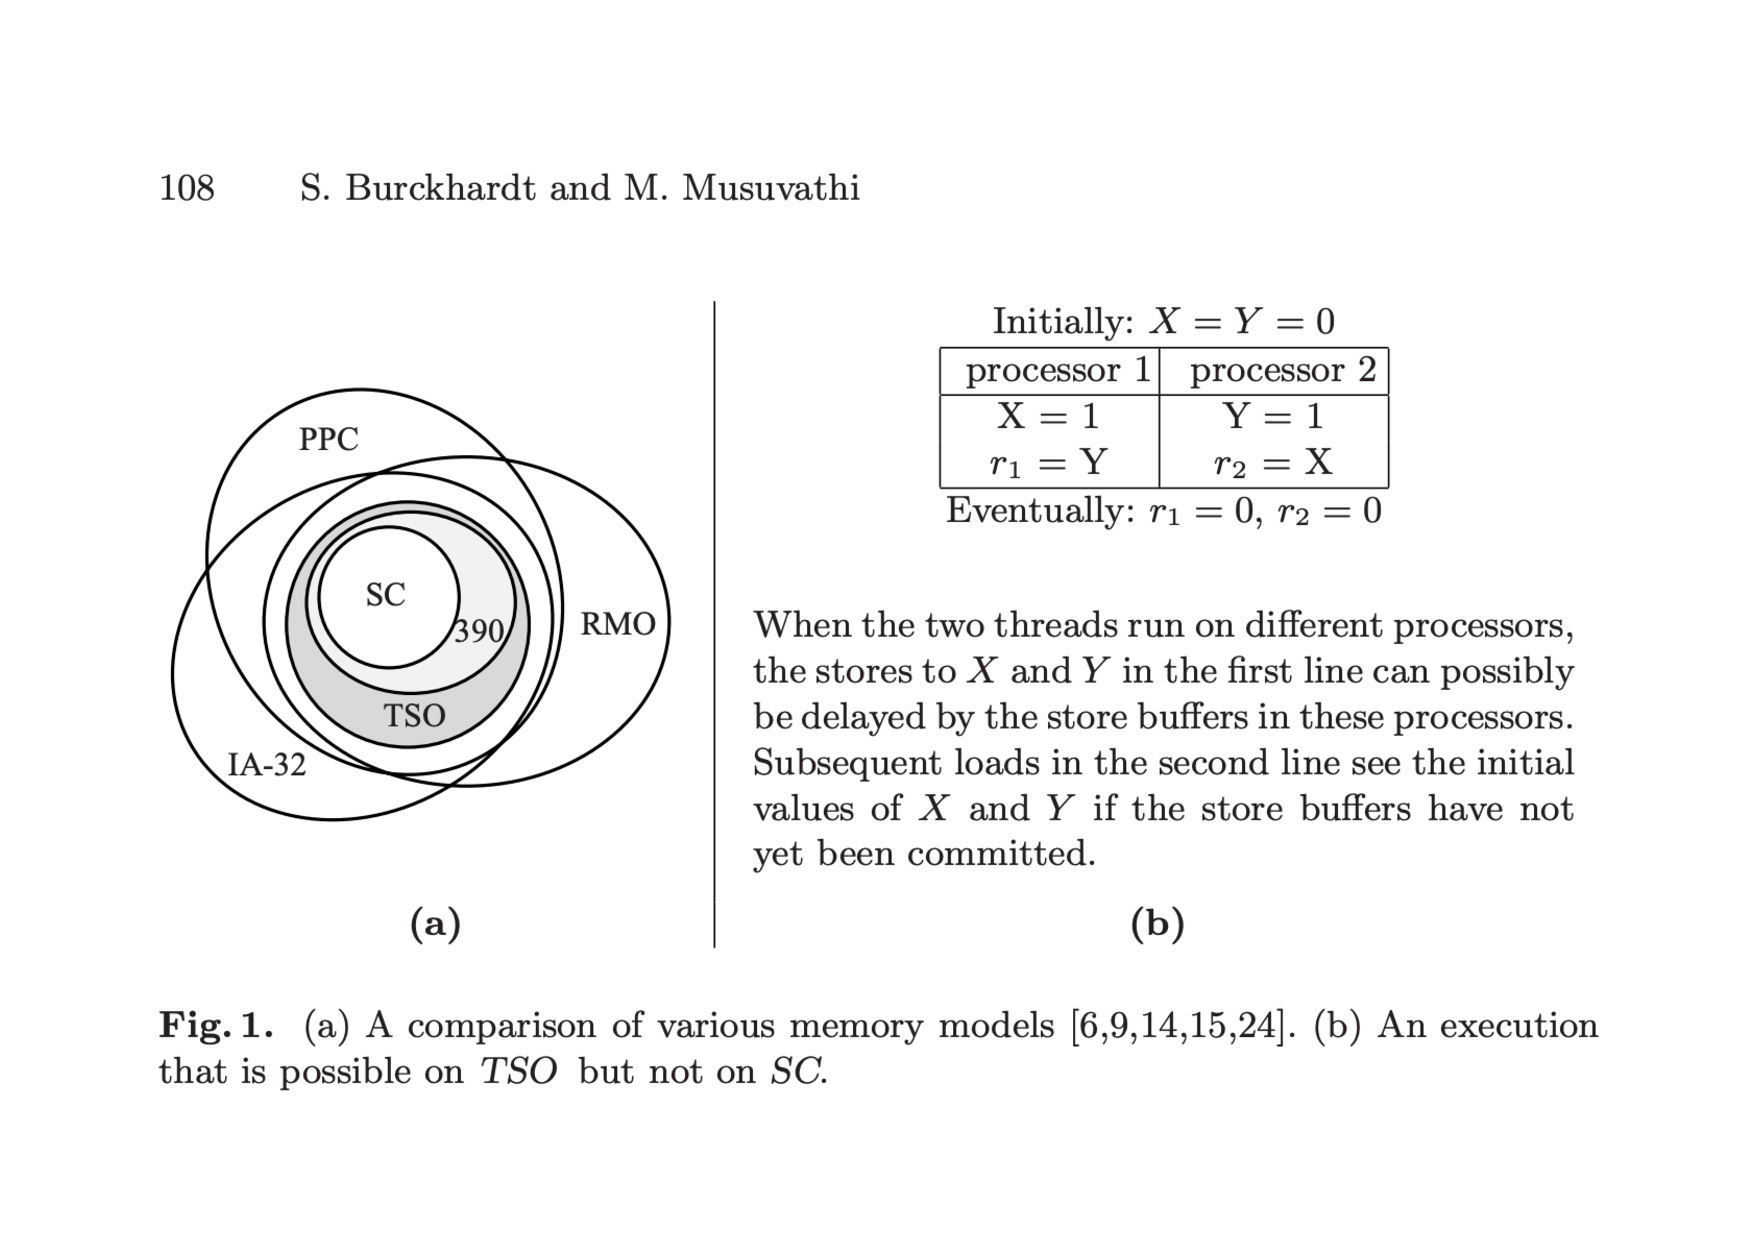
\includegraphics[width=\textwidth]{../images/MModels-and-TSO-vs-SC-BurckhardtM08.pdf}

p107:

Let $\traces_\pi^Y$ denote set of executions of program $\pi$
on memory model $Y$.

p108:

we can sensibly verify the relaxed executions
$\traces_\pi^Y$
by solving the following two verification problems separately:
\begin{enumerate}
  \item
Use standard verification methodology for concurrent programs to show that
the executions in $\traces_\pi^{SC}$ are correct.
2. Use specialized methodology for \emph{memory model safety} verification,
showing
that $\traces_\pi^Y = \traces_\pi^{SC}$ .
We say the program $\pi$ is Y-safe if $\traces_\pi^Y =\traces_\pi^{SC}$ .
\end{enumerate}

$\traces_\pi^{TSO} \subseteq \traces_\pi^Y$ for almost all models $Y$.


\subsubsection{Key Types and Sets}

p110:

\paragraph{Issue Index}
Sequence number relevant to all events by the same processor

\paragraph{Coherence Index}
sequence number of the value that is read or written by the event,
relative to the entire value sequence
written to the \emph{targeted memory location} (my emphasis) during the execution.

\begin{eqnarray*}
   o \in Op &=& \{st,ld,il\} \quad \mbox{store,load,interleave}
\\ p \in Proc &=& \{1,\dots,N\} \quad N \mbox{ fixed}
\\ a \in Adr && \mbox{finite set of addresses}
\\ i \in \Nat && \mbox{issue index}
\\ c \in \Nat_0 &=& \setof{z | z \in \Int, z \not< 0} \quad \mbox{coherence index}
\\ o(p,i,a,c), e \in Evt &=& Op \times Proc \times \Nat \times Adr \times \Nat_0
\\ o(e) &\defs& o' \mbox{ where } e = o'(p,i,a,c)
\\ p(e) &\defs& p \mbox{ where } e = o(p,i,a,c)
\\ i(e) &\defs& p \mbox{ where } e = o(p,i,a,c)
\\ a(e) &\defs& p \mbox{ where } e = o(p,i,a,c)
\\ c(e) &\defs& p \mbox{ where } e = o(p,i,a,c)
\\ E &\subseteq& Evt
\end{eqnarray*}

\begin{eqnarray*}
   E(p) &\defs& \setof{e \in E | p(e) = p}
                \quad \mbox{commands issued by processor }p
\\ L(E) &\defs& \setof{e \in E | o(e) = ld} \quad \mbox{load events }
\\ S(E) &\defs& \setof{e \in E | o(e) = st} \quad \mbox{store events }
\\ W(E) &\defs& \setof{e \in E | o(e) = \in \setof{st,il}}
                \quad \mbox{events that write}
\\ R(E) &\defs& \setof{e \in E | o(e) = \in \setof{ld,il}}
                \quad \mbox{events that read}
\\ W(E,a) &\defs& \setof{e \in W(E) | a(e) = a}
                \quad \mbox{events that write location } a
\end{eqnarray*}

\subsubsection{Traces}

Function $f:Evt \fun \Nat$ is an \emph{index} for $S' \subseteq Evt$
if $f(S') = \setof{1,\dots,|S'|}$.

\paragraph{Traces}

A trace is $E \subseteq Evt$ satisfying:
\begin{eqnarray*}
   \forall p \in Proc &\bullet& i(e) \mbox{ is an index for } E(p) \quad (E1)
\\ \forall a \in Adr &\bullet& c(e) \mbox{ is an index for } W(E,a) \quad (E2)
\\ \forall l \in L(E)
    &\bullet&
      c(l)=0
      \;\lor\;
      (\exists w \in W(E,a(l))\bullet c(l)=c(w)) \quad (E3)
\end{eqnarray*}
Let $\traces \subseteq \Set(Evt)$ be the set of all traces.

Trace $E$ is a prefix of $E'$ if $E \subseteq E'$.

p111:

\paragraph{Order Relations}

\begin{eqnarray*}
   \prgord &\subseteq& Evt \times Evt
\\ e \prgord e' &\equiv& p(e)=p(e') \land i(e) < i(e')
\\ \conflict &\subseteq& Evt \times Evt
\\ e \conflict e'
   &\equiv&
   a(e)=a(e')
   \land
\\ &&\quad (~~(o(e') \in W(Evt) \land c(e)<c(e')))
             \lor
\\ &&\qquad ((e,e')\in W(Evt)\times L(Evt)) \land c(e)\leq c(e') )
\\ \hb &\defs& (\prgord \cup \conflict)
\\ \rhb
   &\defs&
   \hb
   \setminus
   \setof{(e,e')| e \prgord e' \land o(e)=st \land o(e')=ld}
\end{eqnarray*}

\subsubsection{Memory Models}

\begin{eqnarray*}
   \traces^{SC} &\subseteq& \traces
\\ \traces^{SC} &\defs& \setof{ E | \hb \mbox{ is acyclic on } E}
\\ \traces^{TSO} &\subseteq& \traces
\\ \traces^{TSO}
   &\defs&
   \{ E | \rhb \mbox{ is acyclic on } E \quad (TSO1)
\\&& \qquad \forall e,e' \in E \bullet \lnot(e \prgord e' \land p \conflict e')
   \} \quad (TSO2)
\end{eqnarray*}
$TSO2$ guarantees that loads correctly ``snoop'' the store buffer.

\subsubsection{Program Execution}

pp111-112:

\begin{eqnarray*}
   next_\pi &:& \traces \times Proc \fun \Set(Op \times Adr)
\\ next_\pi(E,p) &\defs& \mbox{possible next instructions after } E
\\ last(E,p) &\defs& e \in E(p) |
                     i(e) \mbox{ is maximal, undefined if } E(p)=\emptyset
\end{eqnarray*}

p112:

Program $\pi$ is \emph{locally determinisitic} if
\begin{itemize}
  \item $\forall (E,p) \in \dom~ next_\pi \bullet |next_\pi(E,p)| \leq 1$
  \item $\forall E' \subseteq E
         \bullet
         last(E',p)=last(E,p)
         \implies
         next_\pi(E,p)=next_\pi(E',p)$
\end{itemize}
\textbf{It is assumed at this point that all programs are locally determinisitic}.

\begin{eqnarray*}
   succ_\pi &:& \traces \fun \Set Evt
\\ succ_\pi(E)
   &\defs&
   \{ e \in (Evt\setminus E)
      |
      (E \cup \setof e \in \traces)
      \land
      next_\pi(E,p(e))=(o(e),a(e))
   \}
\end{eqnarray*}

\paragraph{Program Traces}

\begin{eqnarray*}
   \traces_\pi^Y &\subseteq& \traces, \qquad Y \in \setof{SC,TSO}
\\ \emptyset \in \traces_\pi^Y
\\ E \cup \setof e \in \traces_\pi^Y
   &if& E \in \traces_\pi^Y
        \land e \in succ_\pi(E)
        \land E \cup \setof e \in \traces^Y
\end{eqnarray*}

\paragraph{Store Buffer Safety}

Program $\pi$ is \emph{store-buffer safe}
iff $\traces_\pi^{TSO} = \traces_\pi^{SC}$.


\subsubsection{Analysis}

\paragraph{Borderline Trace}

$E \in \traces_\pi^{SC}$ is \emph{borderline}
if $\exists e \in succ_\pi(E)
   \bullet
   E \cup \setof e \in (\traces_\pi^{TSO} \setminus \traces_\pi^{SC})$

Store-buffer safety is equivalent to having no borderline traces.

\paragraph{Cycle Characterisation}

\begin{eqnarray*}
   lastR(E,p)
   &\defs&
   e \in E(p) \cap R(e) |
       i(e) \mbox{ is maximal, or undefined if $\cap$ is empty}
\\ write(E,a,c)
   &\defs&
   e \in W(E,a) |
       c(e)=c \mbox{ if it exists, or undefined otherwise}
\end{eqnarray*}

p113:

Assume
  $E \in \traces_\pi^{SC}$;
  $e = o(p,i,a,c)$;
  and
  $E' = E \cup \setof e$:
\begin{eqnarray*}
   E' \notin \traces_\pi^{SC}
   &\equiv&
   o = ld \land write(E,a,c+1) \hb^* last(E,p)
\\ E' \notin \traces_\pi^{TSO}
   &\equiv&
   o = ld
   \land
   ( (write(E,a,c+1) \rhb^* lastR(E,p))
     \lor
     (\exists c' > c \bullet p(write(E,a,c'))=p))
\end{eqnarray*}

\newpage

p114:

Algorithm to monitor store buffer safety in a given interleaving:
\begin{verbatim}
function is_store_buffer_safe(e1e2 . . . en) returns boolean {
  var k,p,a,c : N; var E : T ;
  E := ∅;
  for (k := 1; k <= n; k++) {
    if (o(ek) = ld) {
      p := p(ek); a := a(ek); c := c(ek);
      while (c > 0) {
        if (p = i(write(E,a,c)))
          break;
        if (write(E,a,c) →∗rhb lastR(E,p))   -- need special algorithm here
          break;
        if (write(E,a,c) →∗hb last(E,p))     -- use 'vector clock' technique
          return false;
        c := c - 1;
      }
    }
    E := E ∪ ek;
  }
  return true;
}
\end{verbatim}

The above algorithm is sound for any interleaving,
and complete over a sufficient set (``representative'') of interleavings.

p116:

vector clock generalised to handle $\rhb$.

\subsubsection{Operational MM}

Also Microsoft tech report (MSR-TR-2008-12)
has some trace automata in an appendix that might be useful.

\paragraph{Trace Automata}

A \emph{trace automaton} over $Evt$ is a tuple
$$
 A = (S,T,initial,accept,guard,apply)
$$
where
\begin{itemize}
  \item $S$ is a set of states
  \item $T \supseteq Evt$ is a set of transitions,
        with $T\setminus Evt$ being considered\emph{internal}.
  \item $initial, accept : S \fun \Bool$ are self-explanatory
  \item $guard : T \fun (S \fun \Bool)$ defines the guard for each transition
  \item $apply : T \fun (S \fun S)$ defines the state-change for each transition
\end{itemize}

A sequence $\omega=\omega_0\dots\omega_n \in T^*$ is accepted by $A$
if there exists $s_0,\dots,s_{n+1} \in S$ such that:
\begin{itemize}
  \item $initial(s_0) = true$
  \item $accept(s_{n+1}) = true$
  \item $guard\seqof{w_i}(s_i) = true$
  \item $apply\seqof{w_i}(s_i) = s_{i+1}$
\end{itemize}
where $ 0 \leq i \leq n$.

\newpage
\paragraph{Sequential Consistency Automaton}

\begin{eqnarray*}
   A_{SC} &=& (S_{SC},T_{SC},initial_{SC},accept_{SC},guard_{SC},apply_{SC})
\\ T_{SC} &=& \setof{st,ld,il} \times Proc \times \Nat \times Adr \times \Nat_0
\\ S_{SC} &=& m : Adr \fun \Nat ;
              i : Proc \fun \Nat
\\ initial_{SC} &=& \forall a,p \bullet m(a)=0 \land i(p)=0
\\ accept_{SC} &=& true
\\
\\ guard_{SC}\seqof{st(p,i,a,c)} &=& i(p)=i-1 \land m(a)=c-1
\\ apply_{SC}\seqof{st(p,i,a,c)} &=& i(p):=i \land m(a):=c
\\
\\ guard_{SC}\seqof{ld(p,i,a,c)} &=& i(p)=i-1 \land m(a)=c
\\ apply_{SC}\seqof{ld(p,i,a,c)} &=& i(p):=i
\\
\\ guard_{SC}\seqof{il(p,i,a,c)} &=& i(p)=i-1 \land m(a)=c-1
\\ apply_{SC}\seqof{il(p,i,a,c)} &=& i(p):=i \land m(a):=c
\end{eqnarray*}
A state-component functions of type $I \fun V$ here
is described in the TR as \texttt{array[\textit{I}] of }$V$.
We use $f(x):=e$ as a shorthand
for function override ($f \oplus \setof{x \mapsto e}$).

\paragraph{Total Store Order Automaton}

We have a FIFO queue, here modelled as a sequence with the following operators:
\begin{eqnarray}
   q \in Q_X &=& X^*
\\ add &:& X \fun Q_X \fun Q_X
\\ add_x(q) &=& q \cat \seqof x
\\ pop &:& Q_X \fun Q_X
\\ pop(\seqof x \cat q) &:& q \quad \mbox{undefined for empty } q
\\ null &:& Q_X \fun \Bool
\\ null(q) &=& q = \seqof{}
\\ peek &:& Q_X \fun X
\\ peek(\seqof x \cat q) &=& x
\end{eqnarray}

\begin{eqnarray*}
   A_{TSO} &=& (S_{TSO},T_{TSO},initial_{TSO},accept_{TSO},guard_{TSO},apply_{TSO})
\\ T_{TSO} &=& \setof{st,st^c,ld,il} \times Proc \times \Nat \times Adr \times \Nat_0
\\ S_{TSO} &=& m : Adr \fun \Nat ;
               i : Proc \fun \Nat ;
               ml : Proc \times Adr \fun \Nat ;
               B : Proc \fun Evt^*
\\ initial_{TSO} &=& \forall a,p \bullet
                   m(a)=0 \land i(p)=0 \land ml(p,a)=0 \land null(B(p))
\\ accept_{TSO} &=& \forall p \bullet null(B(p))
\\
\\ guard_{TSO}\seqof{st(p,i,a,c)} &=& i(p)=i-1
\\ apply_{TSO}\seqof{st(p,i,a,c)}
      &=& i(p):=i \land ml(p,a):=c \land B(p):=add_{st(p,i,a,c)}(B(p))
\\
\\ guard_{TSO}\seqof{st^c(p,i,a,c)} &=& peek(B(p))=st(p,i,a,c) \land m(a)=c-1
\\ apply_{TSO}\seqof{st^c(p,i,a,c)} &=& m(a):=c \land B(p):=pop(B(p))
\\
\\ guard_{TSO}\seqof{ld(p,i,a,c)} &=& i(p)=i-1 \land c = max\setof{m(a),ml(p,a)}
\\ apply_{TSO}\seqof{ld(p,i,a,c)} &=& i(p):=i
\\
\\ guard_{TSO}\seqof{il(p,i,a,c)} &=& i(p)=i-1 \land m(a)=c-1 \land null(B(p))
\\ apply_{TSO}\seqof{il(p,i,a,c)} &=& i(p):=i \land m(a):=c
\end{eqnarray*}
